\documentclass[12pt,letterpaper,oneside,openany]{article}
%\usepackage{Times}
\usepackage{amsmath}
\usepackage{amssymb}
\usepackage{amsthm}
\usepackage{array}
\usepackage{xy}
\usepackage{fancyhdr}
\usepackage{enumerate}
\usepackage[version=3]{mhchem}
\usepackage{graphicx}
\usepackage{caption}
\usepackage{subcaption}
\usepackage{setspace}
\usepackage[super,comma,sort&compress]{natbib}
\usepackage{rotating}
\usepackage{wrapfig}
\usepackage[bottom]{footmisc}
\usepackage{datetime} 
\newdateformat{mydate}{\THEDAY~\monthname~\THEYEAR}

\usepackage{hyperref}

%%%%%%%%%%%%%%%%%%%%%%%%%%%%%%%%%%%%%%%%%%%%%%%
%***************** CUSTOMIZE *****************%

% \usepackage{indentfirst}
\usepackage[top=1.5in, bottom=1in, left=1.25in, right=1in]{geometry}
%\usepackage[margin=1.5in]{geometry}
% \parindent 0.35in

\hypersetup{
    colorlinks,
    citecolor=black,
    filecolor=black,
    linkcolor=black,
    urlcolor=black
}

\pdfpagewidth 8.5in
\pdfpageheight 11in 
%\topmargin 0in
%\evensidemargin 0in
%\oddsidemargin 0in
\headheight 15pt
\headsep 0.25in
\topskip 0in
\textheight 8.5in
\textwidth 6in
\footskip 0.5in
\parskip 0in

\pagestyle{fancy}


\lhead{}
\rhead{}
%\chead{}
%\lfoot{\footnotesize\emph{\today}}
%\cfoot{\footnotesize \emph{Michelle Liu}}
%\rfoot{\thepage}
\renewcommand{\headrulewidth}{0 pt}

% \renewcommand{\sectionname}{Section}

\setcounter{secnumdepth}{1}

%****** ENVIRONMENTS ******%

\renewcommand\abstractname{Abstract}
\renewenvironment{abstract}
{
% \cleardoublepage
 \thispagestyle{empty}
%\null \vfill
\begin{center} \bfseries \abstractname \end{center}}
{\vfill\null}

\newcommand\acknowledgename{Acknowlegments}
\newenvironment{acknowledge}
{\cleardoublepage \thispagestyle{empty}
%\null \vfill
\begin{center} \bfseries \acknowledgename \end{center}}
{\vfill\null}

%***************** END CUSTOMIZE *****************%
%%%%%%%%%%%%%%%%%%%%%%%%%%%%%%%%%%%%%%%%%%%%%%%%%%%


\begin{document}
\author{Tom Bertalan, Michelle Liu\\~ \\CBE 448: Introduction to Nonlinear Dynamics}
\title{Lurching Waves in a Thalamic Neuronal Network}
\date{\mydate\today}

\maketitle


\section{Problem Description}

We wish to model continuous and lurching waves in a thalamic neuronal network using the model described by Wasylenko et al.\cite{Wasylenko2010} The network model contains two types of cells in two separate layers, reticular (RE) cells and thalamocortical (TC) cells. Each RE cell receives excitatory input from $2(\omega+1)$ TC cells and each TC cell is inhibited by just one adjacent RE cell (Figure~\ref{fig:network}).

\begin{figure}[t]
  \centering
  \includegraphics[width=0.6\textwidth]{wasylenkoNetStructure.png}
  \caption{Circular, 1-dimensional array of thalamic neuronal network with two layers of cells, thalamocortical (TC) neurons and reticular (RE) neurons.}
  \label{fig:network}
\end{figure}

We use Wasylenko's 4-equation model for each pair of RE and TC neurons at each site:

\begin{eqnarray}
  \label{eq:ODEs}
C_m \dfrac{dv_i^{TC}}{dt} = -g_L^{TC}(v_i^{TC} - V_L^{TC}) - g_{Ca}(m_{\infty}(v_i^{TC}))^3 \nonumber \\
\times h_i^{TC}(v_i^{TC} - V_{Ca}) - g^{TC}s_{\infty}(v_i^{RE})(v_i^{TC} - V_{syn}^{RE})\\
\nonumber \\
\dfrac{dh_i^{TC}}{dt} = \epsilon^{TC}\left[\dfrac{h_{infty}v_i^{TC}-h_i^{TC}}{\tau_{\infty}(v_i^{TC})}\right]\\
\nonumber \\
C_m \dfrac{dv_i^{RE}}{dt} = -g_L^{RE}(v_i^{RE} - V_L^{RE}) - g_{Ca}(m_{\infty}(v_i^{RE}))^3 \nonumber \\
\times h_i^{RE}(v_i^{RE} - V_{Ca}) - \dfrac{g^{RE}}{2 \omega + 1} \left( \sum_{k=-\omega}^{\omega} s_{\infty}(v_i^{RE})\right)\nonumber \\
\times (v_i^{TC} - V_{syn}^{RE})\\
\nonumber \\
\dfrac{dh_i^{RE}}{dt} = \epsilon^{RE}\left[\dfrac{h_{infty}v_i^{RE}-h_i^{RE}}{\tau_{\infty}(v_i^{RE})}\right]
\end{eqnarray}

where the functions $m_{\infty}$, $h_{\infty}$, $s_{\infty}$, and $\tau_{\infty}$ and associated constants are given in Wasylenko et al. As in the paper, our model used 60 neurons for a total 240-equation system, with $\omega=6$.\cite{Wasylenko2010}

The Wasylenko model was chosen because of its simplicity (only 4 equatios per site in the 1-D network) and because other studies of lurching waves in neuronal networks involved inelegant ``reset'' conditions on neuron voltages after firing.\cite{Golomb1999}

Our goal was to first model the network of neurons described in the paper to observe qualitatively different forms of wave propagation throughout the 1-D network. We then tried to implement continuation techniques to follow branches of solutions and study the transitions between different unstable and stable solutions.

\begin{figure}[t]
  \centering
  \begin{subfigure}[b]{0.5\textwidth}
                \centering
                \includegraphics[width=\textwidth]{wasylenko_waves-s0p60.pdf}
                \caption{s = 0.60}
                \label{fig:waves60}
        \end{subfigure}
        \begin{subfigure}[b]{0.4\textwidth}
                \centering
                \includegraphics[width=\textwidth]{phasespace-s0p60.pdf}
                \caption{s = 0.60}
                \label{fig:phase60}
        \end{subfigure}

        \begin{subfigure}[b]{0.5\textwidth}
                \centering
                \includegraphics[width=\textwidth]{wasylenko_waves-s0p70.pdf}
                \caption{s = 0.70}
                \label{fig:waves70}
        \end{subfigure}
        \begin{subfigure}[b]{0.4\textwidth}
                \centering
                \includegraphics[width=\textwidth]{phasespace-s0p70.pdf}
                \caption{s = 0.70}
                \label{fig:phase70}
        \end{subfigure}

        \begin{subfigure}[b]{0.5\textwidth}
                \centering
                \includegraphics[width=\textwidth]{wasylenko_waves-s0p72.pdf}
                \caption{s = 0.72}
                \label{fig:waves71}
        \end{subfigure}
        \begin{subfigure}[b]{0.4\textwidth}
                \centering
                \includegraphics[width=\textwidth]{phasespace-s0p72.pdf}
                \caption{s = 0.72}
                \label{fig:phase72}
        \end{subfigure}

  \caption{Numerical integration ({\bf a}, {\bf c}, and {\bf e}) and phase portraits ({\bf b}, {\bf d}, and {\bf f}) with different values of the bifurcation parameter 's'}
  \label{fig:numint72}
\end{figure}

\begin{figure}[t]
        \begin{subfigure}[b]{0.5\textwidth}
                \centering
                \includegraphics[width=\textwidth]{wasylenko_waves-s0p71.pdf}
                \caption{s = 0.71}
                \label{fig:waves71}
        \end{subfigure}
        \begin{subfigure}[b]{0.4\textwidth}
                \centering
                \includegraphics[width=\textwidth]{phasespace-s0p71.pdf}
                \caption{s = 0.71}
                \label{fig:phase71}
        \end{subfigure}
  \caption{Numerical integration ({\bf a}) and phase portraits ({\bf b}) with 's' = 0.71}
  \label{fig:quasiper}
\end{figure}

\section{Numerical Integration}


We used direct time integration in Python study the possible solutions as we change the bifurcation parameter, 's', over the range of values used in Wasylenko et al.\cite{Wasylenko2010} The results are shown in Figure~\ref{fig:numint}.

In all of the space-time plots (Figure~\ref{fig:numint} {\bf a}, {\bf b}, and {\bf c}), we see a wave representing the voltages of the TC neurons. As 's' is varied from 0.60 to 0.72 we observed that the behavior of the waves also changed. For lower values of 's', the behavior is almost like a continuous chain of neurons because the ``perturbation'' introduced by this small discretization is low. This is a ``smooth'' wave, or a ``1-lurcher''. At $s=0.70$ the system starts to exhibit transient lurching behavior---the transient part of the solution appears to be almost quasiperiodic, but then settles down to a smoother wave. Above that, around $s=0.72$ the lurching is persistent and is a true 6-lurcher.

The phase portraits in $V^{TC}$-$V^{RE}$ space show the trajectories that the neurons in the lattice follow. For the smooth wave, all of the neurons follow the same path. Though we did not plot Poincar\'{e} maps, we would expect there to be only one fixed point in the map, indicating a stable limit cycle. For the transient lurcher, we observe that the phase portrait contains more than one path, but the paths are not clearly separated. If we were to integrate for more time we would expect to see the paths converge, and we would expect the Poincar\'{e} map to approach a closed curve indicative of a torus solution. For the stable 6-lurcher, there are six separate paths in the phase plane even after long integration times. The Poincar\'{e} map would show six discrete points.

In Figure~\ref{fig:numint71}, 's' is set to an intermediate value between lurching and transient, where 's' = 71. To the eye, it appears as if solution will continue lurching indefinitely, but the phase portrait associated with it seems to hint that is actually near the beginngs of a toral solution.

\section{Continuation}

We used continuation techniques in AUTO with FORTRAN in order to study the bifurcations of stable and unstable solutions as the parameter 's' is varied. However, we were not able to get the AUTO and FORTRAN files to follow a branch of solutions.

Rather than implementing the period-shift Poincar\'{e} map used in Wasylenko et al.\cite{Wasylenko2010}, we opted for a map which integrated over the entire network of neurons for the ``true'' period for feasibility of coding. However, we would want to inplement the period-shift code eventually in order to make the calculation more efficient.

Our continuation methods allowed us to visualize only one quilibrium point before terminating with no convergence (Figure~\ref{fig:EP}). Further debugging is needed to determine why the continuation protocol does not diverge. However, we were able to plot solutions for the voltages and gating variables through AUTO, as well as obgain a plot in phase space which looked similar to those obtained in Python and in Wasylenko et al.\cite{Wasylenko2010}

We suspect that part of the problem with our AUTO code is specifying the correct period length in AUTO. The constants in the AUTO constants file likely also need to be optimized in order to follow the branch of solutions.

\begin{figure}[t]
  \centering
  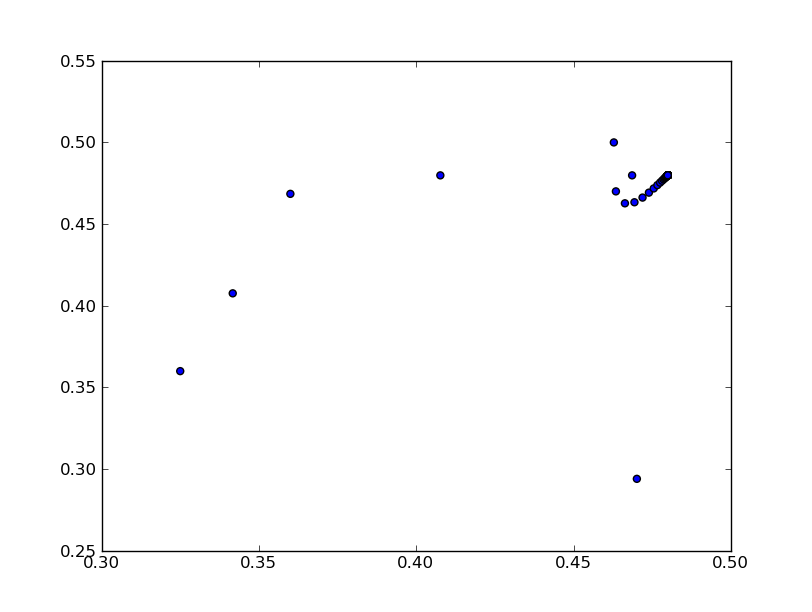
\includegraphics[width=0.5\textwidth]{4dNOPE.png}
  \caption{Poincar\'{e} map of the 3-lurcher. This map was meant to be similar to Figure 4d of Wasylenko et al. However, the points do not appear to fall on a closed curve on the map. This is likely due to remaining bugs in the code.}
  \label{fig:4dNOPE}
\end{figure}

\begin{figure}[t]
  \centering
  \includegraphics[width=0.5\textwidth]{VRE.png}
  \caption{Solution for a RE neuron.}
  \label{fig:VRE}
\end{figure}

\begin{figure}[t]
  \centering
  \includegraphics[width=0.5\textwidth]{VTC.png}
  \caption{Solution for a TC neuron.}
  \label{fig:VTC}
\end{figure}

\begin{figure}[t]
  \centering
  \includegraphics[width=0.5\textwidth]{hRE.png}
  \caption{Solution for $h_{RE}$.}
  \label{fig:hRE}
\end{figure}

\begin{figure}[t]
  \centering
  \includegraphics[width=0.5\textwidth]{hTC.png}
  \caption{Solution for $h_{TC}$.}
  \label{fig:hTC}
\end{figure}

\begin{figure}[t]
  \centering
  \includegraphics[width=0.5\textwidth]{EP.png}
  \caption{The only point of interest found during our AUTO run. It is still unclear why AUTO stopped after finding this equilibrium point.}
  \label{fig:EP}
\end{figure}

\begin{figure}[t]
  \centering
  \includegraphics[width=0.5\textwidth]{phase.png}
  \caption{Plot in $V_{TC}$-$V_{RE}$ phase space.}
  \label{fig:phase}
\end{figure}




% \newpage
% \appendix

% \section{Numerical Integration Files}
% \label{sec:numAppendix}
% File: wasylenko.py

% \begin{verbatim}



% \end{verbatim}

% \section{Continuation Files}

% blah blah

\bibliography{448}
\bibliographystyle{unsrt}
\end{document}